\documentclass[conference]{IEEEtran}
\IEEEoverridecommandlockouts
% The preceding line is only needed to identify funding in the first footnote. If that is unneeded, please comment it out.
\usepackage{cite}
\usepackage{amsmath,amssymb,amsfonts}
\usepackage{algorithmic}
\usepackage{graphicx}
\usepackage{textcomp}
\usepackage{xcolor}
\def\BibTeX{{\rm B\kern-.05em{\sc i\kern-.025em b}\kern-.08em
    T\kern-.1667em\lower.7ex\hbox{E}\kern-.125emX}}
\begin{document}

\title{Segmentation and background detection for human identification\\
}

\author{\IEEEauthorblockN{1\textsuperscript{st} Mikel-ange Barros}
\IEEEauthorblockA{\textit{computer science department} \\
\textit{University Claude Bernard Lyon 1}\\
Lyon, France\\
mikel-ange.barros@etu.univ-lyon1.fr}
\and
\IEEEauthorblockN{2\textsuperscript{nd} Zacharia Beddalia}
\IEEEauthorblockA{\textit{computer science department} \\
\textit{University Claude Bernard Lyon 1}\\
Lyon, France \\
zacharia.beddalia@etu.univ-lyon1.fr}
}

\maketitle

\begin{abstract}
Image processins is  a set of fundamental researc in areas of image pattern based recognition.
In this research, Segmentation methods are the core to analyze the given Image
This document present our method of segmentation and this use for a body detection in a video.
In this paper, we will show you our method and part of code, and we will compare it to other existing method.
\end{abstract}

\begin{IEEEkeywords}
segmentation, body detection
\end{IEEEkeywords}

\section{Introduction}
Image analysis is a branch of computer science with increasing application, whether in the field of video games, medicine or data protection. All of its technologies use an image segmentation method, setting up new segmentation methods adapted to these different applications is therefore an important part of the work to be carried out. our work is therefore moving in this direction in order to obtain convincing results in the detection of moving human bodies on a video

\section{Image Segmentation}

Image Segmentation is the first stage of processing an image. For the segmentation to be deemed effective, many criteria must be met. Among these criteria, we can notably note the speed of execution as well as the precision of the detected zones.  As I have said, Image Segmentation is an important field of image analysis and for a better comprehension of it  image segmentation is Classified in foor type :

\begin{itemize}
\item Segmentation by edges detection : This type of  segmentation try to detect the the contours of different objects in order to identify them. In this type of segementation, we can notice : Canny's edges detections.
\item Segmentation by thresholding : This type of  segmentation try to detect the the colour of differents objects in order to identify them. With this technique, we will try to separate an object in a color spectrum of the rest of the objects. In this type of segementation, we can notice : Adaptive thresholding techniques.
\item Segmentation by  region based: This type of segmentation try to detect regions composed of pixels  with the same characteristics. In this type of segementation, we can notice :  Single Seeded Region Growing.
\item Segmentation by Feature Based Clustering : This type of segmentation try to detect cluster composed of pixels  with the same characteristics. The differences with the Segmentation by region based  is that a cluster is not necessarily composed of adjacent pixels, unlike a region. In this type of segementation, we can notice :  K-means Algorithm.
\end{itemize}

In this Paper, the methods used is a Single Seeded Region Growing. We will compare it to a K-means Algotithm and a wattershed algorithm, implemented by the library opencv.

\subsection{Single Seeded Region Growing}

This segmentation method is based on a selection of random pixels. Thus, during the execution of this algorithms, a certain number of pixels will be selected in order to serve as a center for our region. Once these points have been selected, the algorithm will make the regions magnify by processing the pixels around the region. A pixel with similar characteristics is added to the region and removed from the list of available pixels.  After this phase, regions with similar characteristics and being side by side are merged together.

This type of algorithm is usually applied to a grayscale image.


\subsection{OpenCV K-means algorithm}

In order to be able to execute this algorithm, we must first define the number of clusters with which the image will be cut out. After this has been done, the algorithm will place points, called the center of the cluster, and will add the pixels of the image to the clusters while trying to minimize a function.
In order to be able to execute this algorithm, we must first define the number of clusters with which the image will be cut out. After this has been done, the algorithm will place points, called the center of the cluster, and will add the pixels of the image to the clusters while trying to minimize a function.

This type of algorithm is usually applied to a color image.

\subsection{OpenCV watershed algorithm}

In principle of this algorithm, each grayscale image can be seen as as a heightmap where high intensity denotes peaks while low intensity denotes valleys. You start filling every isolated valleys with different colored water (labels). As the water rises, depending on the peaks nearby, water from different valleys, obviously with different colors will start to merge.  However, we do not want all regions to merge.
For this, OpenCv implements an algorithm or have defined in advance that they will be the zones which can merge and which cannot. For this, we use a first segmentation by edge detection.

This type of algorithm is usually applied to a grayscale image.

\section{Our Algorithm}

\subsection{Basic principle}

As I told you above, our algorithm is based on the principle of a single seeded region growing. As defined above, we will therefore randomly place points on an image, these points will serve as bases for the rest of the algorithm. The main difference between our algorithm and a classic algorithm is that our algorithm is applied to a color image.

\subsection{Data structure}

To implement this algorithm we need a data structure to store information. As our algorithm is based on a region-based algorithm, it seemed logical to use a data structure based on a region principle. Thus, we define each zone of our segmented images as being a structure containing all the pixels of the region, all the neighbors of the region, all the borders of the region and the average color of the pixels belonging to the region. 
Thanks to this structure we can easily interact on our region, create and modify them which will serve us for the future, the region growing.

\subsection{Region growing}

In order to start our region growing, we need to define the points on which our regions will be centered. For this, we randomly generate a number of points defined by the user and we create as many regions as there are points. We then assign a point to each region and this point will serve as the basis for the enlargement of our regions. In order to define that a point in a region has already been processed, each of the points already visited is kept and marked as visited. 
Once this has been defined, we can move on to the main loop of our region growing. We therefore loop over all the regions and at each iteration for a pixel in the region, we look at the 8 neighboring pixels. For each of the neighboring pixels: 
\begin{itemize}
\item If this neighbor is already marked by another region we add this other region to the list of neighbors of the region and the pixel is added to the border of the region.
\item if this neighbor is marked by ourselves, we do nothing 
\item if this neighbor is not marked then we calculate the distance between the color of the pixel belonging to the region and the color of the pixel that we want to add to the region. If this region is at a distance below a user-defined threshold then it is added to the region, otherwise it is added to the border of the region.
\end{itemize}

This part of the algorithm stops when all the regions no longer get bigger.

At the end of our region growing , we calculate the average color of the region's pixels and store it for use in our region merging.


\subsection{Region merging}

In this part of our code, we will merge all similar and neighboring regions. For this, we are going for each region, look for each of its neighbors if they have a similar average color. To do this, we calculate the Euclidean distance between the two colors and see if it is below a threshold. If the two regions have similar colors, then we merge them. Once a region has been merged, it is deleted and will therefore no longer be able to absorb other regions.

When all the regions have been processed then we quit the execution and we can display the segmented image.


\subsection{Comparative result}

As explained above, we compare the results obtained by our algorithm to the result of a k-means algorithm and to those of a watershed algorithm. First, we can see that the different zones are fairly well recognized by our algorithm (b) and the k-means algorithm (c). We can also notice that the watershed  (d) does not seem to adapt to the analysis of an image of this type. We will therefore exclude this algorithm for the following steps.
Now looking at the last two algorithms, we can notice that the kmeans to less clean and less smooth regions algorithm than our algorithm. And that, despite the fact that the kmeans algorithm makes it possible to segment the image in more detail, our algorithm makes it possible to identify the general shapes of objects with more precision, which is more suitable for detecting human bodies in the basic image (a).

\begin{figure}[h!]
  \centering
  \begin{tabular}{@{}c@{}}
    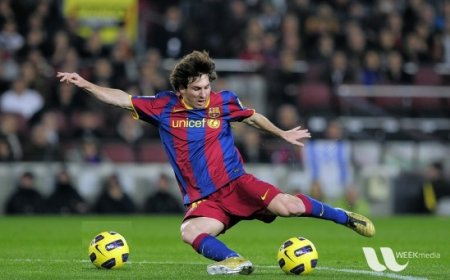
\includegraphics[width=0.4\linewidth]{fig0.jpg} \\[\abovecaptionskip]
    \small (a) basic image
  \end{tabular}
  \begin{tabular}{@{}c@{}}
    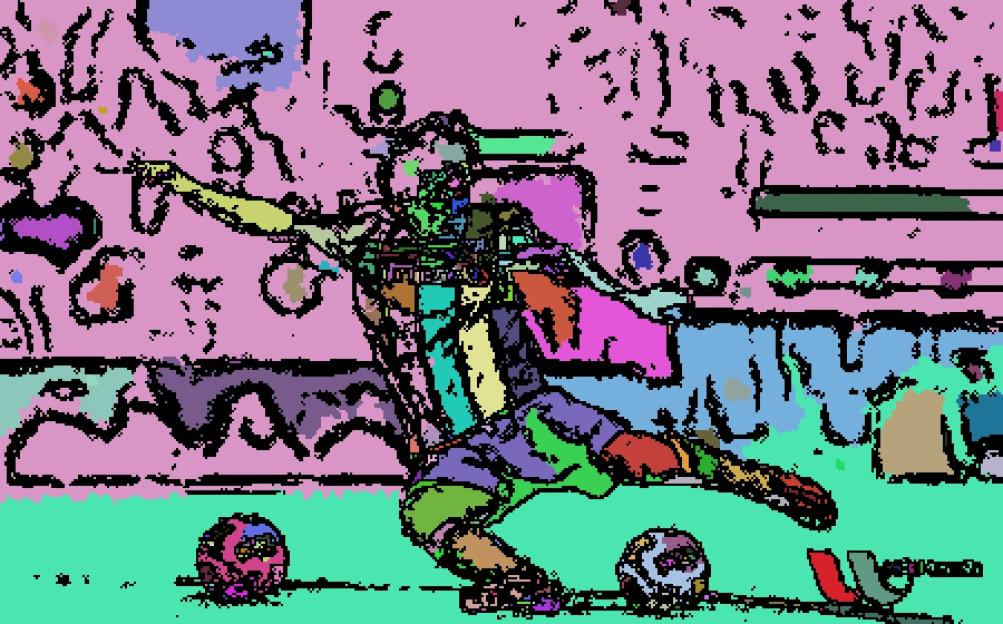
\includegraphics[width=0.4\linewidth]{fig1.jpg} \\[\abovecaptionskip]
    \small (b) our result
  \end{tabular}

  \vspace{\floatsep}

  \begin{tabular}{@{}c@{}}
    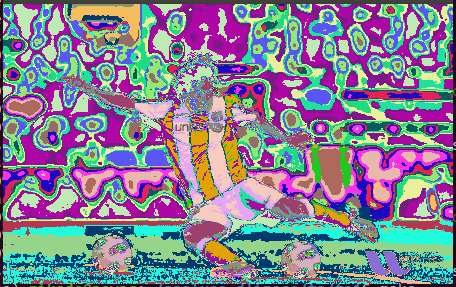
\includegraphics[width=0.4\linewidth]{fig2.png} \\[\abovecaptionskip]
    \small (c) k means result : 32 cluster
  \end{tabular}
  \begin{tabular}{@{}c@{}}
    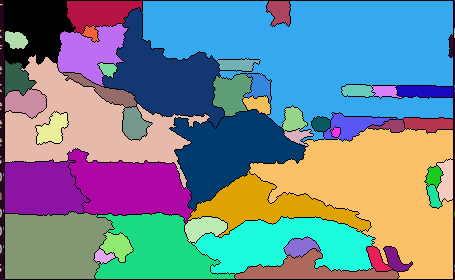
\includegraphics[width=0.4\linewidth]{fig3.png} \\[\abovecaptionskip]
    \small (d) watershed result
  \end{tabular}
  \caption{comparative results}
  \label{fig 1}
  
\end{figure}

\section{Background Detection}

In order to allow background detection on videos, OpenCV provides two tools, the first being the backgroundDetector class and the second being the motion detection classes. After different tests it seemed to us that the results returned by the two classes were very similar and as the movement detection was faster at execution we decided to use this class.

\subsection{Movement detection}
 
The OpenCV movement class implement two method to analyse the movement , the lucas Kanade algorithm and the Gunnar Farneback’s algorithm. The Gunnar Farneback’s algorithm seems to be the most suitable for character detection because it allows to surround the moving area. But before proceeding with an analysis of the movement, we must first eliminate the noise which risks being identified as being a moving part on the video. For this, we use the OpenCV function: fastNlMeansDenoisingColored which will remove the noise on a color image.
With this allgorithm we manage to identify the moving elements and cut out the background elements, from the basic image (a), useless for our body detection.
After this movement detection, we obtain a result (b)  with the body cuted from the background, but a part of the background is cut with. To eliminate this identification defect, we use the segmentation seen in the first part.

\begin{figure}[h!]
  \centering
  \begin{tabular}{@{}c@{}}
    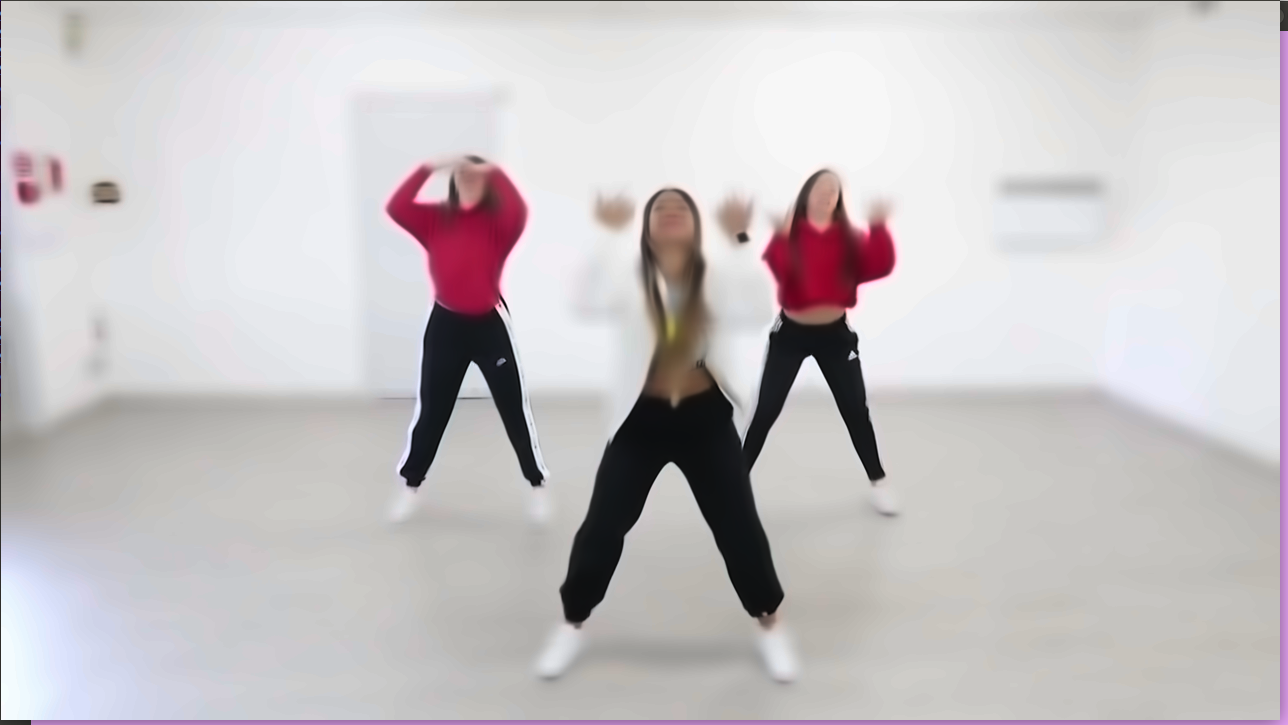
\includegraphics[width=0.4\linewidth]{fig5.png} \\[\abovecaptionskip]
    \small (a) basic image
  \end{tabular}
  \begin{tabular}{@{}c@{}}
    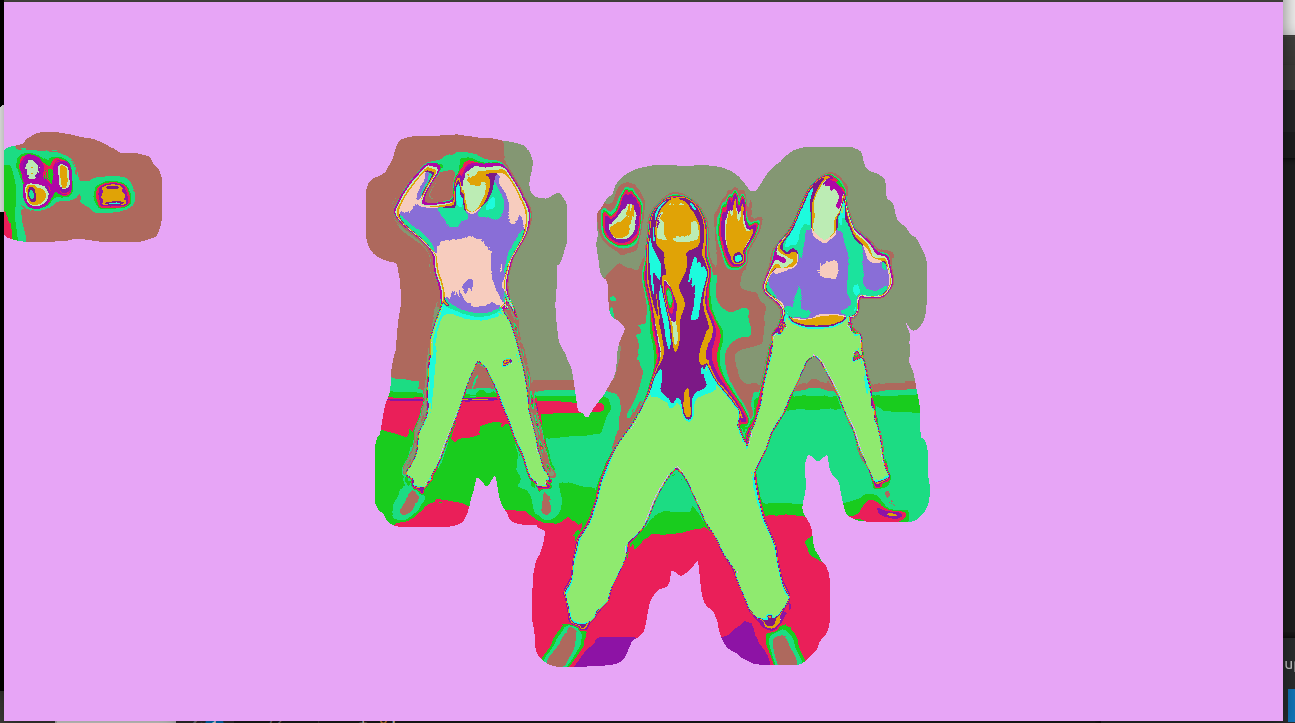
\includegraphics[width=0.4\linewidth]{fig6.png} \\[\abovecaptionskip]
    \small (b) movement detection result
  \end{tabular}
  \caption{Movement detection}
  \label{fig 2}
\end{figure}

\subsection{Segmentation and body detection}

\section*{Acknowledgment}

Thanks to Ms. Saida for this project end her help.

\section*{References}



\vspace{12pt}
\color{red}

\end{document}
